\chapter{Background} \label{background}

This work describes the approach to, and algorithms for finding exact solutions to the \aspop{}. Some context for the problem, along with some details of our intended applications for it are explored in Section \ref{context} below. Section \ref{solving_ASPOP} details the starting point for the \gls{suffix filter} algorithm from the literature used in the final implementation of our solver. These \glspl{filter algorithm} are complex by nature. As such, the final algorithm is incrementally \textit{approached} by solving simpler, related problems listed in \ref{relevant}. This incremental explanation spans sections \ref{solving_P1} - \ref{P3_suff}.

\section{Context}
\label{context}

An \aspop{} solver has a number of applications in the field of Bioinformatics. Arguably, the most common application is as part of a genome assembly pipeline designed to iteratively agglutinate overlapping reads into chains until the full genome is acquired.

Our work is primarily interested in developing an \aspop{} solver as part of the assembly of viral DNA. Viral DNA has a number of properties not ubiquitous to DNA in general, such as more modestly-sized genomes. Often the solver is intended to distinguish between numerous \gls{source genome} \textit{strains} mixed into the data set. Such strains have much in common for viral DNA; As such, they have very many runs of identical nucleotides. To tell one strain from another, it makes sense to ignore extremely short overlaps, as a significant proportion of short overlaps are expected between different strains. To reduce the discovery of these deceiving solutions, valid overlaps  only with with lengths above 80-100 nucleotides are retained, considered `likely enough' to be from overlaps within the same strain. For the purpose of this work, whenever necessary, this value is pinned down to 80. To compensate for the diminished solution set resulting from discarding overlaps, generally data sets for viral DNA contain a significant number of \glspl{genome copy} (Data sets with a high degree of \gls{coverage}), generally in the range of 10 000x to 100 0000x. At the moment, such an assembly problem simply involves too many reads for our existing \aspop{} solvers to deal with at a time, leading to runaway time and space requirements. A viable workaround involves partitioning the original data set into a \textit{set} of smaller problems the \aspop{} solver can manage, then combining results later down the assembly pipeline. It is our hope that a more efficient \aspop{} solver can reduce the granularity of this partitioning, or better yet, avoid it entirely.

\section{Relevant Problems}
\label{relevant}

Understanding the nature and solutions to simpler problems than \aspop{} serve to incrementally approach our implemented algorithm in its final state. The explanations in this section refer to these problems. For the sake of specificity, the set of these problems is laid out in Table \ref{tab:related} with their definitions; For the sake of brevity, they are assigned short monikers that are used to refer to them in Sections \ref{solving_P1} - \ref{P3_suff}.



\begin{table}[H]
\centering
\caption{Problems discussed in the text, given short monikers and their relations to one another described.\strut}
\begin{tabularx}{\textwidth}{|s|s|b|m|}
\hline

Moniker & Name  & Description & Relevance \\
\hline
\hline


P1 & Pair Within Distance  & Return whether two given strings, $\bfit{A}$ and $\bfit{B}$, are within a given $\bfit{K}$ error distance of each other. & The simplest problem.  \\
\hline

P2 & Approx. String Match & Given a whole number $\bfit{K}$, a \textit{\gls{text}} string and a \textit{\gls{pattern}} string, return all substrings of the pattern that are within ~$\bfit{K}$ error distance of the pattern. & Return all substrings of the pattern that return \textit{true} when used as P1 instances.\\
\hline

P3 & Approx. Prefix Match & Return the indices within a given \bfit{text} string of matches $B$ of all strings $A$, where $A$ is any prefix longer than a given whole number $\bfit{t}$ of a given $\bfit{pattern}$ string, and the error rate of the match from $A$ to $B$ is no larger than a given~$\bfit{e}$. & An instance of P2 for every prefix with length at least~t of the pattern.  \\
\hline

\aspop{} & Approx. Suffix-Prefix Overlap & Return all approximate overlaps at least given integer \bfit{t} long between the prefix of $A$ and the suffix of $B$, where $A$ and $B$ are any strings in the given set $\bfit{S}$; The overlap must have an error rate no larger than a given $\bfit{e}$. & An instance of P3 for each string in $S$ as the pattern. Additionally, solutions are restricted to occurring as suffixes of $S$ strings.  \\ \hline
\end{tabularx}
\label{tab:related}
\end{table}
% \end{table}

\section{Solving P1: Pair Within Distance}
\label{solving_P1}

Checking whether two given strings are within a certain \gls{error distance} is a well-known problem. In the case of \gls{Hamming distance}, it is simply the count of \glspl{mismatch} between symbols compared pairwise between the given strings for all the string indices.
 
In the case of \gls{edit distance}, much extensive work exists. Edit distance (here shortened to `ed') between strings $X$ with length $x$ and $Y$ with length $y$ can be defined recursively:
% //
% \vspace{1mm}
\[ 
\text{    ed(X,Y)} = min\left \{
\bgroup
\def\arraystretch{2}
\begin{tabular}{p{6.2cm}|p{3cm}}

ed($X[1,x]$, $Y[1,y-1]$) + 1
&\gls{insertion} case
\\
% \hline
ed($X[1,x-1]$, $Y[1,y]$) + 1
&\gls{deletion} case
\\
% \hline
ed($X[1,x-1]$, $Y[1,y-1]$) + z
\newline{}
where $z=1$ if $X[x]\neq{}Y[y]$ else 1.
&\gls{substitution} or match case
% \\

\end{tabular}
\egroup
\right \}
\]
% \vspace{2mm}

A well-known dynamic programming solution builds a table incrementally, with each cell storing the edit distance between unique pairs of prefixes of the input strings. Further optimizations exist to avoid populating the entire table, but they are beyond the scope of this work.








\section{Solving P2: Approximate String Match}
\label{solvingP2}


P2 is the problem explored by \kark{} in~\cite{kark2007}. More difficult than P1, P2 can be naively decomposed into numerous instances of P1 subproblems. However, this is not the only approach possible. By using a \gls{text index}, a much smarter algorithm can find the same \glspl{solution} in less time by leveraging the shared work done for different possible \glspl{derived string} of the same string. However, as demonstrated by the \glspl{filter algorithm} to come, use of an index alone could still be considered naive.




\subsection{Solving P2 Using a Text Index} \label{P2text_index}

Finding all exact instances of a given string inside a \gls{text} is the job description of a \gls{text index}, designed to quickly locate occurrences of a given \gls{query} string within the prepared text. It is then only a matter of extending their functionality to find \glspl{approximate match} within the text by considering \glspl{derived string} producible from the query string by permitting \glspl{error}. A number of well-researched text indices exist which are suitable for this purpose. Our work uses a version of the \textit{FM-Index} with a simulated forward-search procedure. For more details on indices and the FM-Index in particular, see Section \ref{aux_info}. For more details on the simulated forwards search, see Section \ref{own_impl_search_dir}.
 
The FM-Index makes use of an iterative search procedure for exact occurrences of a given query\footnote{We find that considering the text index a black-box that interacts with the rest of the system in a call-response fashion a useful metaphor for understanding the nature of the search. As such, `query' refers to whatever full string the text index is searching for, with the set of match locations returned being the `response'.} string, iterating over symbols in the query one at a time while keeping track of \glspl{match location} inside the text every step of the way. Intuitively, this process begins with a set of match locations (initialized as the full range of the text), and gradually thins the set out. Throughout the search, match locations mark text substrings \textit{equivalent} to the prefix\footnote{Although this holds conceptually, in practice, this matching occurs in reverse (matching longer suffixes instead). This is discussed further in Section \ref{own_impl_search_dir}} of the query string matched so far. If no match locations remain, the search terminates. If the entire query string is matched, match locations are returned, representing occurrences of the query string within the text.
 
The idea behind the \gls{K-approximate} search is to generate all possible $K$-approximate derivations of the A string recursively. To achieve this, the search begins provided a new parameter \bfit{pE} (for `permitted errors'), initialized to $K$. As before, query symbols are considered one at a time, at each step narrowing down the set of match locations (and representing an incrementally-longer matched prefix of the query). However, instead of pruning matches that differ from the query string, when the \bfit{pE} parameter allows, the search retains match locations that \gls{mismatch} with the next query symbol, `spending' a permitted error (decrementing \bfit{pE}) for those match locations. As the search considers all match locations in batches, it needs to associate appropriate \bfit{pE} values for each match location; As shown in fig \ref{fig:index_search}, this is achieved by recursively branching the search for each symbol, partitioning the remaining match locations and pruning branches with empty match location sets.


\begin{figure}[!h]
\centering
\tikzset{
  treenode/.style = {align=center, inner sep=0pt, text centered,
    font=\sffamily},
  arn_n/.style = {treenode, circle, white, font=\sffamily\bfseries, draw=black,
    fill=black, text width=2.2em},% arbre rouge noir, noeud noir
  arn_r/.style = {treenode, circle, red, draw=red, 
    text width=2.2em, very thick},% arbre rouge noir, noeud rouge
  arn_x/.style = {treenode, rectangle, draw=black,
    minimum width=0.5em, minimum height=0.5em}% arbre rouge noir, nil
}

\begin{tikzpicture}[->,>=stealth',level/.style={sibling distance = 3cm/#1,
  level distance = 1.1cm, scale=1.2}] 
\node [arn_n] {$\epsilon$}
    child{ node [arn_n] {T} 
            child{ node [arn_n] {TT} 
            	child{ node [arn_n] {TTC} edge from parent node[above left]
                         {exact match}} %for a named pointer
							child{ node [arn_r] {TTT}}
            }
            child{ node [arn_r] {TC}
            		child{ node [arn_r] {TCC}}	
            }                            
    }
    child{ node [arn_r] {C} 
            child{ node [arn_r] {CT} 
              	 	child{ node [arn_r] {CTC}}
            }
		}
; 
\end{tikzpicture}
\caption[Search tree of 1-approximate matching.]{Search tree for 1-approximate matching of `TTC' using a text index with alphabet $\{T, C\}$. Black nodes have \bfit{pE}$=1$ and red nodes have \bfit{pE}$=0$.}
\label{fig:index_search}
\end{figure}

In practice, further unique branches are generated for each newly-matched symbol, as by the nature of the FM-Index, it is only possible to retain a subset of the match locations according to a \textit{specific symbol} at a time. 



Branches of the $K$-approximate search that reach the end of the query string represent \glspl{exact match} for strings \textit{derived} from the query (analogous to \textit{approximate} matches for the query). These leaf nodes each return return a set of match locations, the union of which represent the solution set of the problem.







\subsection{Solving P2 Using Substring Filters} \label{p2substring}

A \gls{substring filter} algorithm can be employed to reduce the search space of P2. The correctness of the \gls{filter criterion} is reliant on lemma \ref{lemma1}, originally provided by \kark{}, where it was called `Lemma 1.1'~\cite{kark2007} .

\begin{lemma}
\label{lemma1}
If a string containing no more than $K$ symbols $\phi{}$ is partitioned into $K+1$ blocks, at least one block must have $0$ $\phi{}$'s.
\end{lemma}

Term $\phi{}$ is any arbitrary symbol, but we consider the case when $\phi{}$ refers to an \gls{error} in the \gls{derivation} from some other string $X$. These errors occur at index positions and fall into partition \glspl{block} as any symbol would. Lemma \ref{lemma1} is based on something akin to the pigeonhole principle. As the \gls{string partition} also partitions the set of errors, the lemma observes that with more blocks than errors, there must be at least one block without any errors at all. 

To satisfy the precedent of the lemma, the substring algorithm begins by partitioning the given \gls{pattern} into $K+1$ blocks for a given \textit{error limit} argument $K$. A \gls{text index} is built for the \gls{text} as before. Now, instead of querying the index for all approximate instances of the entire $A$ string monolithically (as described in Section \ref{P2text_index}), the algorithm instead performs a \textit{set} of \glspl{query}. For each block of the pattern's partition, the index is queried for \glspl{match location} of just that single block in the text, allowing for no errors whatsoever. For each location of a complete block in the text found this way (with no errors all the way to the end), a \gls{candidate} is generated to mark a possible occurrence of an \gls{approximate match} of the pattern.

Each block’s query yields a set of candidates and the union of these sets is called the \textit{candidate set}. Observe that thanks to lemma \ref{lemma1}, as long as every pattern block is queried, any actual \gls{K-approximate} matches of the pattern string must bring rise to a candidate in one or more block's queries; The candidate set \textit{covers} the solution set. However, it does not hold that every candidate is a \gls{solution}; Candidates are generated to represent overlaps involving some substring occurrent at a match location in the text; However, the symbols of blocks \textit{adjacent} to this substring's blocks are not checked at all; They might be fraught with errors, or be predicted to extend beyond the bounds of the text. Finding the subset of candidates that are also solutions is done by iterating over candidates, retaining only candidates that satisfy the \gls{solution criterion}, `verifying' them to be solutions. This \gls{verification step} can be solved as an instance of P1.
 
The substring filter algorithm reduces cost by taking measures \textit{likely} to reduce the search space; Some cases don’t save time at all. Consider the following P3 problem:
\begin{align*}
\text{pattern}  &= \text{`GGGG'}\\
\text{text} &= \text{`GGGGGGGGGGG'}
\end{align*}

Approaching this instance with substring filters would produce a storm of candidates as very many \glspl{exact match} of pattern blocks will be found. In such a case, the filter provides no utility at all, and the algorithm degenerates to something akin to naively considering all possible derivations at all possible locations in the text. Thankfully, in practice, the majority of realistic problem instances have sparser solutions than the example above, and more effectively filter the search space.
 
Note the correctness of the algorithm is defined for arbitrary pattern partitions, so long as there are at least $K+1$ partition blocks. However, the manner in which the pattern is partitioned contributes significantly to computational cost. Consider the following instance with partitions already chosen:
\begin{align*}
\text{pattern:  } P &= `0000111101'\\
P_1 &= `0000' & P_2 &= `1111' & P_3 &= `01'\\
\text{text} &= `0101010101'
\end{align*}

Although this text certainly contains no matches of this pattern, it \textit{does} contain very many occurrences of the entirety of $P_3$, generating 5 \textit{spurious} candidates. Circumstances of this nature become more probable with short pattern blocks.







\subsection{Solving P2 Using Suffix Filters}
\label{P2suffix}

The \gls{suffix filter} algorithm described by \kark{} is quite similar to the \gls{substring filter} algorithm described in Section \ref{p2substring} above. The difference lies with its efforts to have a stricter \gls{filter criterion}, such that some more time is spent in the \gls{search step} generating a smaller set of \glspl{candidate}, and much less time is spent in the \gls{verification step}. The \gls{solution} set remains unchanged from the other P2 algorithms described so far.
 
The correctness of the suffix filter algorithm relies on lemma \ref{lemma2}, paraphrased from \kark{}'s paper, where it is called `Lemma 2.1'~\cite{kark2007}.


\begin{lemma}
\label{lemma2}
Consider only non-empty \glspl{block sequence}. If a string has a partition $Z$ with more blocks than symbols $\phi{}$, in at least one of $Z$'s \glspl{suffix block sequence} $S_Z$, for all \glspl{prefix block sequence} $P_{SZ}$ of $S_Z$, the number of blocks in $P_{SZ} >$ the number of $\phi{}$'s in $P_{SZ}$.
\end{lemma}

Lemma \ref{lemma2} can be understood as a natural consequence of Lemma \ref{lemma1}, applying under the same conditions but making a different observation. Assuming the premise holds, it guarantees for at least one suffix block sequence $S_Q$ of the pattern string, $Q$, the following is true:
When iterating over blocks in any prefix block sequence $P_{SQ}$ of $S_Q$ from left to right, there will always be strictly fewer cumulative errors encountered in $P_{SQ}$ than cumulative blocks counted.
 
To understand why lemma \ref{lemma2} holds, consider walking over all partition blocks of the string from left to right, counting encountered \glspl{error} at each block (inclusively). As there are fewer errors in total than blocks, at some stage during the iteration the cumulative number of errors must fall behind the index of the current block, never to catch up. It is at this moment that the suffix block sequence with the desired property begins. This `walking' description is rather suggestive of how the lemma is actually applied in the \gls{search step}.

As with the substring filter algorithm, the suffix filter algorithm begins by constructing a \gls{text index} for the given text string. The given pattern is again partitioned into $K+1$ blocks; However, where before \glspl{query} were performed for each pattern \textit{block}, the suffix filter algorithm performs a query for each \textit{suffix block sequence} of the pattern instead; The difference is outlined in Figure \ref{fig:substring_vs_suffix}.

\begin{figure}[!htb]
\centering
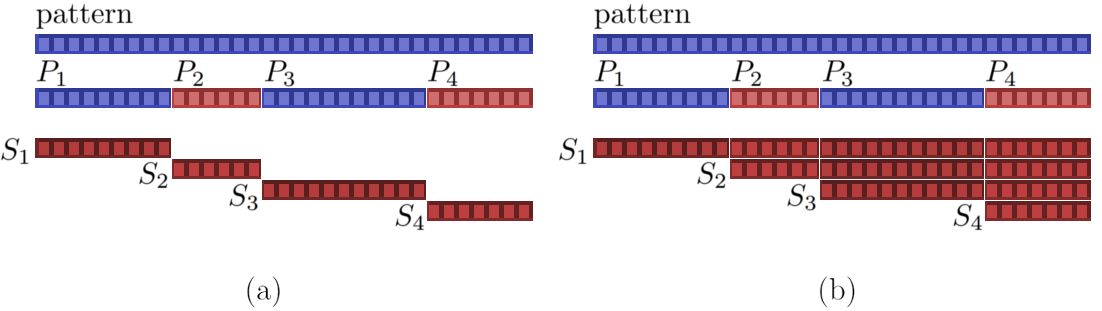
\includegraphics[width=1.0\textwidth]{images/substring_suffix.png}
\caption[Pattern string blocks vs. suffix block sequences for substring and suffix filter algorithms.]{Pattern string partitioned into blocks $[P_1, P_2, P_3, P_4]$, bringing rise to sequence of queries $[S_1, S_2, S_3, S_4]$. (a) Queries of the substring filter algorithm, one query per block of $P$. (b) Queries of the suffix filter algorithm, one query per suffix block sequence of $P$.}
\label{fig:substring_vs_suffix}
\end{figure}

As in the substring filter algorithm, the search process walks over query symbols one by one, keeping track of incrementally-longer \gls{match location} sets in the text throughout. Only now, the query string is comprised potentially of numerous blocks instead of just one. The search makes use of a parameter \bfit{pE} as it did in the indexed P2 algorithm, but this time it is initialized at $0$, effectively prohibiting any error-branching at first. Every time the search walk crosses over the end of a block, the search \textit{accumulates} a permitted error (i.e. incrementing \bfit{pE} by one); This alteration to the procedure effectively results in a limited version of the recursive branching seen in the indexed P2 algorithm from Section \ref{P2text_index}.

\begin{figure}[!htb]
\centering
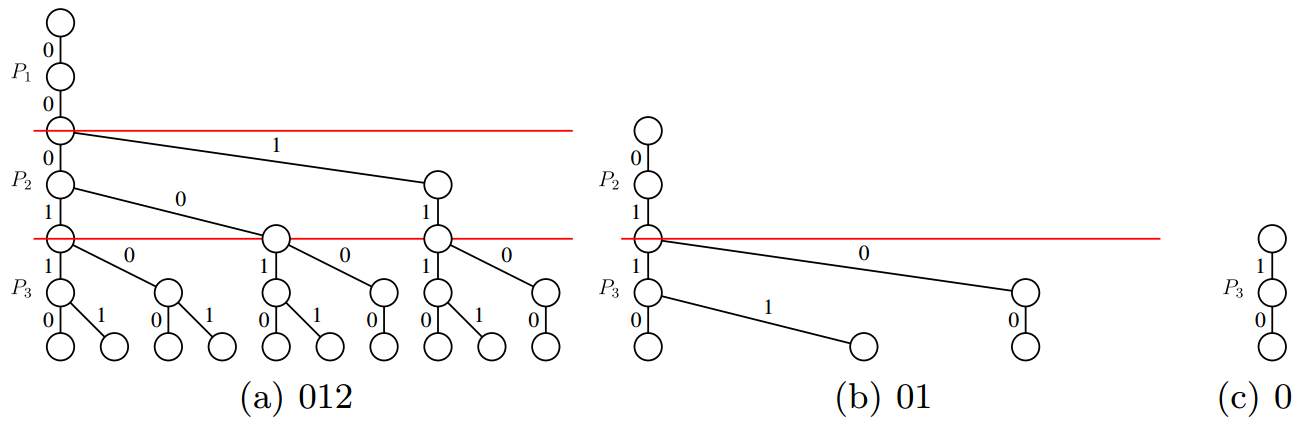
\includegraphics[width=0.92\textwidth]{images/trie.png}

\caption[Search trees from pattern `000110' using a binary alphabet, bringing rise to filters 012, 01 and 0 and three blocks, $P_1, P_2, P_3$]{Search trees\protect{}\footnotemark{} from pattern `000110' using a binary alphabet, bringing rise to filters 012, 01 and 0 and three blocks, $P_1, P_2, P_3$ (a) 3-block query for `100110' using filter 012. (b) 2-block query for `0110' using filter 01. (c) 1-block query for `10' using filter 0.}
\label{fig:filter_search}

\end{figure}
\FloatBarrier
\footnotetext{This Figure is taken from Kucherov \cite{kuch2014}}

% This algorithm relies on lemma \ref{lemma2} much like the substring filter algorithm relied on \ref{lemma1}; The lemma guarantees that for an arbitrary solution's match in the text $Y$, for at least one query, the branching behavior described above should be \gls{sufficiently lenient} such that it can match symbols all the way to the end of the pattern without eliminating the \gls{match location} for $Y$ from the set. As such, upon reaching the end of the the query string, the search generates a \gls{candidate}. Unlike the previous algorithm, many branches of the search tree may find their own such candidate sets. The return result of such a query is the union of all these sets.
 
The correctness of the suffix filter algorithm relies on the \textit{consequent} of lemma \ref{lemma2}. An arbitrary search query is \textit{not} guaranteed to find an arbitrary string $Y$ in the text; However, the lemma guarantees that \textit{at least one} search query for a suffix block sequence will have enough errors to spare throughout the search all the way to the end of the matching substring with $Y$ in the text, where it would generate a candidate to cover the \gls{solution} containing $Y$. As with the substring P2 algorithm, not all candidates necessarily correspond to solutions, as the search is `blind' to the symbols in blocks that prefix the first block of the query.
 
Observe that the suffix filters conduct a more \textit{thorough} search process, with blind sections for matches only on \textit{one} side, instead of on \textit{both} sides as was the case with substring filters. The suffix filter algorithm generally produces far fewer candidates, as it searches further to potentially thin out the match location sets than the substring filter algorithm does before generating candidates. Also observe that the \gls{search step} of the suffix filter algorithm takes longer, as it needs to spend more time searching more symbols \textit{with} recursive branching. In this sense, the suffix filter algorithm makes more extensive use of the text index than the substring filter algorithm.
\section{Solving P3: Approximate Prefix Match Using Suffix Filters}
\label{P3_suff}

Problem P3 is closely related to P2. However, instead of the \gls{pattern} being fixed, given as an argument directly, matches are found for any string $A$ that is any prefix of a given \gls{pattern} at least as long as the given \bfit{t}. At first glance, extending the \gls{suffix filter} algorithm for P2 seems simple; Indeed, the problem can be solved with several instances of P2 separately, one for each \textit{valid} prefix of the pattern playing the role of P2's input `pattern' (where `valid' is shorthand for `at least as long as \bfit{t}'). Although perfectly correct, this approach does not take advantage of the similarity between the prefixes; The beginnings of the \gls{text index} search \glspl{query} would repeat many of the same steps, duplicating work. Instead, \glspl{candidate} for each prefix can be located \textit{in tandem} without altering correctness; However, some care is required to preserve the premises of lemmas \ref{lemma1} and \ref{lemma2} on which the suffix filter algorithm is built.

% As described several times since section \ref{P2text_index}, throughout the search procedure of the text index, incrementally-longer prefixes of the query are \textit{matched}. Now, i

 
Instead of separate P2 problems, P3 can be approached as being more like a single instance of P2, where partially-completed query matches during the search may also represent desirable candidates (some nodes in the search tree mark the end of valid query prefixes). To implement this idea, the search procedure must be able to generate candidates when its progress corresponds with any \gls{derived string} of a valid query prefix.

During an index search, the degree to which the search node at an index position increments \bfit{pE} is a function of the sizes of the pattern's blocks; This requires the partition block sizes to be defined \textit{prior} to the search query's commencement. However, the correctness of the algorithm is reliant on every valid pattern prefix $A$ being divided into at least $K+1$ blocks, where $A$'s have various lengths and thus various values for $K$. This requires a single initialization for partition block sizes that sufficiently partitions all pattern prefixes finely enough at the same time. Although this is tricky conceptually, the partition can still be defined in terms of the pattern itself, as the \textit{error limit} for each of its prefixes is a predictable linear function of the prefix lengths (excepting for some rounding). This is the idea behind \vali{}'s \gls{partitioning scheme}; It seeks to identify a value \bfit{p}, the length of all pattern blocks (except for the last block, which can be smaller) such that no valid pattern prefix $A$ will have too few blocks and \bfit{p} is maximal. Kucherov's work describes their own partitioning scheme that satisfies this property, but distributes block lengths differently. These details are further explained in Section \ref{schemes}.


This algorithm for P3 is where the P2 `filter-free' text index algorithm from Section \ref{P2text_index} gets left in the dust. For long patterns, the text index search algorithm would need to permit very large initial values for \bfit{pE}, resulting in very deep and wide recursive search trees, branching far more than would be necessary to match the short prefixes of the patterns, but unable to avoid doing so in order to find the solutions for longer prefixes. The filter algorithms are able to leverage the \textit{incremental} introduction of \bfit{pE} to great effect for this reason, allowing for a much more appropriately \textit{gradual} introduction of errors, resulting in slimmer search trees.





\section{Solving the Approximate Suffix-Prefix Overlap Problem Using Suffix Filters}
\label{solving_ASPOP}

Where before the search space was defined by a given \gls{text} string, now the search space is defined by a given \textit{set} of strings $S$. Allowing for some bookkeeping steps before and afterwards, the \gls{text index} can be made to search these strings by being initialized with a text constructed from concatenated $S$ strings. Although it would cover all the solutions, unmodified, the above approach is too generous, as it would naively generate \glspl{candidate} anywhere within the constructed text (even overlapping two different $S$ strings). \Glspl{solution} would only exist as suffix positions for individual strings of $S$. Detecting these suffix positions is trivial if the text string is constructed with some distinct extra-alphabetic character delimiting the concatenated $S$ strings (conventionally `\$'). For example:
\begin{align*}
S &= \{\text{`TACC'}, \text{`GGG'}, \text{`ACCC'}\}\\
\text{text} &= \text{`TACCGGGACCC'}
\end{align*}

During the \gls{search step}, at the moment where the search is about to generate candidates from \glspl{match location}, an additional `\$' symbol is matched, effectively narrowing down the match location set to a subset that occur as $S$ suffixes; Only for all the match locations in this subset are candidates generated. The original match location set at this position remains unchanged and potentially continues the forward search, generating more candidates deeper into the search tree.
 
Aside from the alterations described in Section \ref{extensions} to support extensions, the above is the basis for the algorithms used to solve the \aspop{} onwards in the paper. As such, the \gls{suffix filter} solution to the \aspop{} as described in this section will henceforth be referred to as the `\aspop{} algorithm' for the `\aspop{} solver'.


\section{Suffix Filtering and Partitioning Schemes} \label{schemes}

\Glspl{suffix filter} allow a much faster search than the filter-free \gls{text index} search, and filter more thoroughly than \glspl{substring filter}, saving a lot of time in the \gls{verification step}. For these to result in an exact algorithm, the premises of the lemmas on which they are based need to be satisfied. This introduces requirements for the implementation of the \gls{filter criterion}, the \gls{partitioning scheme} of the \gls{pattern}, and determines when \glspl{candidate} must be generated throughout the \gls{query} searches to ensure to \glspl{solution} are missed. However, these requirements only \textit{bound} the possibility space for these algorithms, but do not specifically \textit{define} it; Design decisions arise that impact run time but not correctness. For instance, the suffix filter algorithm is only guaranteed to find all solutions when the patterns are divided into at least $K+1$ \glspl{block}. Partitioning into $K+2$ blocks satisfies the requirement, but profoundly changes the number of the text index \glspl{query}, the shape of each search tree, et cetera. Different choices for these design decisions result in different \textit{schemes}, many of which are explored thoroughly by \vali{} and Kucherov in an attempt to maximize speedup.



\subsection{Filtering Scheme Defined}
\label{schemes:def}

The \gls{search step} of any \gls{filter algorithm} is tasked with partitioning the search space into elements that satisfy the \gls{filter criterion} (\glspl{candidate}) and those that do not. How this set of candidates is \textit{found} is a matter that depends on the specific problem and its nature.
 
For \glspl{suffix filter}, elements in the search space, nodes in the search tree and string \glspl{derivation} of \gls{query} strings are all equivalent; Which branches are explored in a search determines the search elements encountered. For this reason, there is not complete freedom to use any branching behavior, but (as discussed in Section \ref{P3_suff}) the rules that ultimately determine branching need to be established such that they satisfy lemmas \ref{lemma1} and \ref{lemma2} to guarantee no solutions are overlooked. However, several conceivable such `branching behaviors' satisfy the lemmas. A \gls{filtering scheme} for the suffix filter algorithm defines a \gls{filter} for each query string's \gls{block sequence}, where a filter is simply a sequence of integers. During the search, each query block is associated with one filter value; Upon the search entering a new block, it uses the block's \textit{filter value} $fE$ to determine if and how much to increment \bfit{pE}, such that $sE+\bfit{pE}=fE$, where $sE$ is the error `spent' on the search node so far\footnote{As all \bfit{pE} could conceivably be spent at any time, by implication the numbers in a filter sequence are strictly \textit{nondecreasing} in the order they are encountered by the search.}. In this way, the contents of the filters define the branching behavior of query searches.

{the filter specifies a number for each block, interpreted as the maximum possible \bfit{pE} value entering that block during the search.
 
Consider the algorithm described in Section \ref{P3_suff} with some pattern $P$ divided into 3 blocks, and the search of the longest of $P$’s \glspl{suffix block sequence} (all 3 blocks) with filter $\{0, 1, 2\}$. The resulting search would initialize \bfit{pE} to 0, and increment \bfit{pE} by 1 at each subsequent block; This should look familiar, as it is the same scheme described in \ref{P3_suff}; This is \kark{}'s filtering scheme:

\begin{fscheme}[Karkainnen's Filters]
\textup{For a pattern with N blocks}
\label{karkfilters}
\begin{align*}
filters &= \{f_0, f_1\ldots{} , f_N\}\\
f_X &= [0, 1, 2,\ldots , X-1]
\end{align*}
\end{fscheme}


\subsection{Partitioning Scheme Defined}
The \gls{suffix filter} algorithms in this work have various requirements for the number of \glspl{block} in a \gls{string partition}; Indeed, even the one existing requirement for partition block sizes (discussed in Section \ref{P3_suff}) was only required to indirectly ensure a sufficient \textit{number} of blocks for all prefix strings. With this detail accounted for, the algorithms have no requirements on the \textit{size} of blocks. However, the shape of the search tree for a \gls{query} is a function of block sizes. For this reason, the choice of how a \gls{pattern} is partitioned greatly impacts cost of a suffix filter algorithm, and the rules that define these choices are called a \gls{partitioning scheme}.




\subsection{\kark{}'s Schemes}
\label{schemes:kark}

The \kark{} \glspl{suffix filter} had an efficient \gls{partitioning scheme}, suited for the problem they sought to solve (P2: `Approximate String Match' in Section \ref{solvingP2}), a simpler problem than the ASPOP. In their case, the length of the \gls{pattern} was known from the start. For this reason, the \gls{string partition} of pattern could be chosen to greedily minimize search time for that pattern and be the best choice overall.

For the \textit{substring filter} algorithm, the optimal string partition is obvious. As each \gls{filter} simply matches a single \gls{block}, the best speed is achieved with evenly-sized blocks. However, for \glspl{suffix filter} the choice is less clear, as evenly-distributed blocks do not result in work being evenly-distributed amongst filters.

\kark{} observed that \glspl{query} that started in a short block had fewer opportunities to narrow down their \glspl{match location} before starting to generate \glspl{candidate} (once the first block was completely matched), which manifested in such queries generating storms of spurious candidates. These factors suggested that a good scheme required a balance to be struck between \textit{preventing short blocks} (a pressure to evenly-distribute block lengths) and to \textit{balance the work of each filter} (a force to make the right-most blocks longer than the left-most blocks). \kark{} opted to make the \textit{last} block longer than the rest, with the other $K$ blocks dividing up the remaining length as evenly as possible. \kark{} observed that this alteration to the partitioning scheme had a positive effect on the runtime of the algorithm, but they could not find a trivial way of optimizing the choice of length for the last block, resigning it to be determined experimentally on a case-by-case basis.


\subsection{\vali{}'s First Schemes}
\label{schemes:vali1}

The first \vali{} paper attempted to most-directly adapt \kark{}'s \gls{suffix filter} algorithm for the \aspop{}, using filtering scheme \ref{karkfilters} (\kark{}'s filters).

\vali{} recognized the potential of searching all prefixes of strings in parallel and were forced to adapt the \gls{partitioning scheme} in accordance to the new correctness constraints imposed by this choice (as described in Section \ref{P3_suff}). To ensure every \textit{valid} prefix was divided up into at least $K+1$ blocks, \vali{}'s approach provides a formula to determine the largest choice for uniform block length that would not overlook any prefixes for the given \gls{pattern} size. Keeping block lengths largely uniform was carried over from the \kark{} implementation. This was a logical choice to always increment \bfit{pE} at the last possible moment in the search in order to minimize the width of the search tree. As identified by \kark{} in their own work, this design had an optimally-short \gls{search step}, but created very many spurious \glspl{candidate} that would increase time taken in the \glspl{verification step}. The use of a predefined block size presented a problem when used for the \aspop{}; Very many indices in the pattern (in fact all indices larger than \bfit{t}) correspond with the end of some \textit{valid} prefix; For simultaneous searches for all prefix matches (as described in \ref{P3_suff}), a prefix might end part-way through some pattern block, cutting that block short; This is shown in Figure \ref{fig:short_block}. When seen in isolation, such a prefix would have a short final block (in the worst case, the final block would be only 1 symbol long!) and the final filter would generate many spurious candidates. This situation arises in every partitioning scheme with any block division occurring after \bfit{t}.

\begin{figure}[!htb]
\centering
\makebox[\linewidth][c]{%
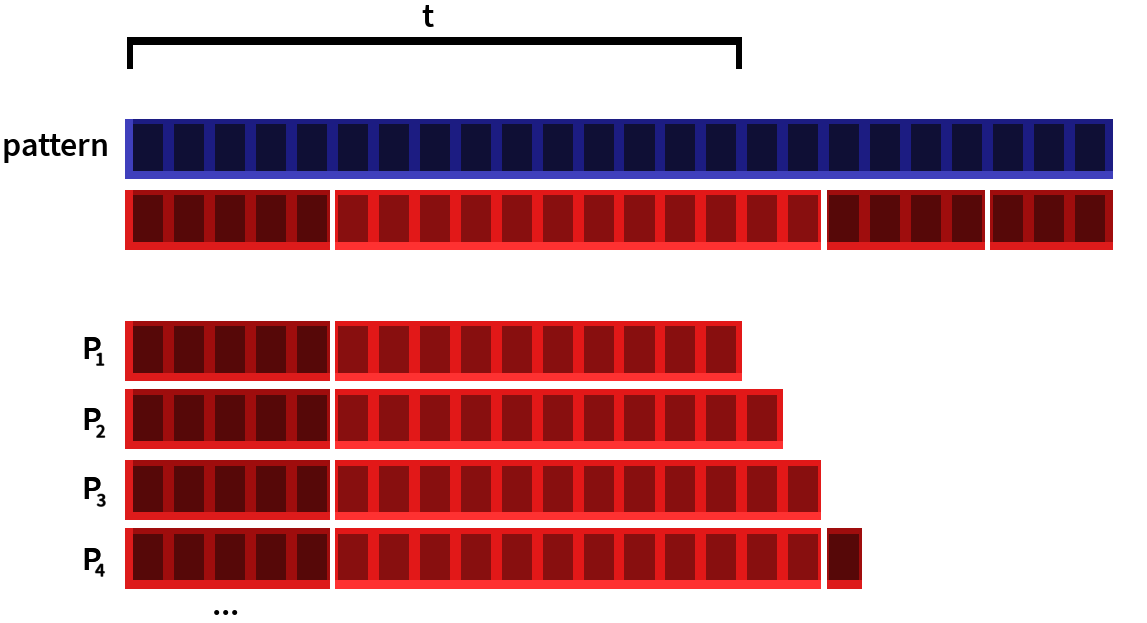
\includegraphics[width=0.7\textwidth]{images/short_block.png}
}
\caption[Short final block in some prefix of a pattern demonstrated]{Prefixes $P_1...P_4$ of some pattern string, where the length of $P_4$ induces a short final block from the pattern's block sequence.}
\label{fig:short_block}
\end{figure}
 
To remedy this problem, \vali{} had a number of ideas which involved passing over the same prefix a number of times, each time offsetting the partitioning divisions on the pattern, and selectively disabling candidate generation whenever these short blocks were predicted to arise. Without dwelling too much on the specifics, this approach was able to cumulatively cover all \glspl{solution} and avoid having to output candidates in cases with extremely short queries. However, it required several passes over the same pattern.





\subsection{\vali{}'s Second Schemes}

\label{schemes:vali2}
Following up their previous paper, \vali{} proposed a new \gls{filtering scheme} to sidestep the problem of short \glspl{block} that plagued their previous algorithm.
 
\begin{fscheme}[Valimaki's Filters]
\textup{For a pattern with N blocks}
\label{valifilters}
\begin{align*}
filters &= \{f_1, f_2\ldots{}, f_{(N-1)}\}\\
f_1 &= [1, 2,\ldots , N]\\
where\phantom{ }X \neq 1 : f_X &= [0, 1, 2,\ldots, X-1]
\end{align*}
\end{fscheme}

\noindent
The new filtering scheme had a new desirable property; To cover all \glspl{solution} for any \gls{pattern} of $K+1$ blocks, the very shortest \gls{filter} (composed of a single block) could be entirely omitted. For the algorithm, this meant that a solution for any prefix of the pattern would be covered even if all searches did not generate \glspl{candidate} until the end of the complete first block. The new algorithm was able to output candidates in just one \gls{text index} \gls{query} per filter. To cover cases that would ordinarily only be found by the missing \gls{query}, the first (largest) \gls{filter} that all prefixes would have in common has its \bfit{pE} 1 larger in all positions than in filtering scheme \ref{karkfilters}; This can be achieved in the search by initializing $\textit{pE} = 1$ instead of 0, giving the branching a head start. As a consequence of the wider search tree, more time is spent in the \gls{search step}. However, the increase in search time is vastly outweighed by the \textit{decrease} in time spent in the \gls{verification step} when using filtering scheme \ref{karkfilters}.






\subsection{Kucherov's Schemes}
\label{schemes:kuch}

In the fashion of \vali{}'s second paper, Kucherov attempted to make an improvement to the earlier algorithm of \vali{}'s first paper by fixing the short first \gls{block} problem. Kucherov offered a new \gls{filtering scheme} that achieved this in a new way.

\begin{fscheme}[Kucherov's Filters]
\textup{For a pattern with N blocks, given a positive integer $S$}
\label{kuchfilters}
\begin{align*}
filters &= \{f_0, f_1\ldots{}, f_{(N+S-1)}\}\\
f_X &= [0, 1, 2,\ldots , X-S]
\end{align*}
\end{fscheme}

Instead of each prefix having $K+1$ partition blocks (for error limit $K$), Kucherov's solution relies on $K+S$ blocks for each prefix, with $S\geq2$. This could be interpreted as guaranteeing $S$ error-free blocks up from just one. This change increases the breadth of search trees, but avoids many \textit{spurious} candidates from being generated, thereby saving time in the \gls{verification step}; The key observation is that the unavoidable \textit{short last block} can now no longer be the \textit{only} block matched for any candidate; Hence, no candidate will be generated with less than one \textit{complete} block's worth of symbols matched.

The correctness of this algorithm can be seen from lemma \ref{lemma0}, a more generalized version of lemma \ref{lemma1}.

\begin{lemma}
\label{lemma0}
If a string containing no more than $K$ symbols $\phi{}$ is partitioned into $K+S$ blocks for $S \geq 0$, at least $S$ blocks must have $0$ $\phi{}$'s.
\end{lemma}

In Kucherov’s canonical example, $S=2$ (where $S=1$ in \vali{}’s first algorithm), but any positive value of $K$ remains correct. With more finely-partitioned prefix patterns, the \gls{filtering scheme} could safely assume that each \gls{solution} would contain more \gls{error}-free blocks, and match more blocks before generating \glspl{candidate}. So far, the assumption of the 0-error blocks occurring as the \textit{first} block in each query only holds because queries are generated to exhaustively guarantee the correctness of the algorithm \textit{using all} queries (essentially branching into a \textit{case distinction} for which each case covers one position for the 0-error block). Creating queries relying on the \textit{specific} position any \textit{subsequent} 0-error blocks in the \gls{block sequence} (for example, the 2nd of two for $S=2$) would require \textit{another} layer of case-distinction, resulting in a number of filters and queries quadratic in the number of blocks, rather than linear. To avoid this, the position of subsequent blocks is not nailed down at all, and \bfit{pE} continues to be incrimented until the last possible moment; In effect, this simply requires that 0-error blocks number 2 to $S$ occur \textit{somewhere} in the block sequence after the first 0-error block. This reasoning is based on lemma \ref{lemma2}.

In addition to guaranteeing more complete blocks matched per candidate, increasing $S$ results in more balanced (albeit increased) work across filters. In a sense, small values of $S$ cause the algorithm to approach the \kark{} algorithm, while large values of $S$ cause it to degenerate towards the filter-free \gls{text index} algorithm from Section \ref{P2text_index}; (The advantage of using blocks at all falls away as blocks get shorter.)
 
In the previous filtering schemes with uniformly-increasing \bfit{pE}, \glspl{filter} of all lengths were prefixes of one another. This is not the case for these Kucherov filters. For searches intended to traverse all prefix lengths (and thus, apply all lengths of \gls{suffix filter}) in tandem, this requires the search path to \textit{fork} at each new block, with some branches accruing an extra \bfit{pE}, and others matching $S-1$ blocks, generating candidates and terminating. Figure \ref{fig:pE_fork} demonstrates this branching search path for $S = 2$. 


\begin{figure}[!htb]
\centering
\makebox[\linewidth][c]{%
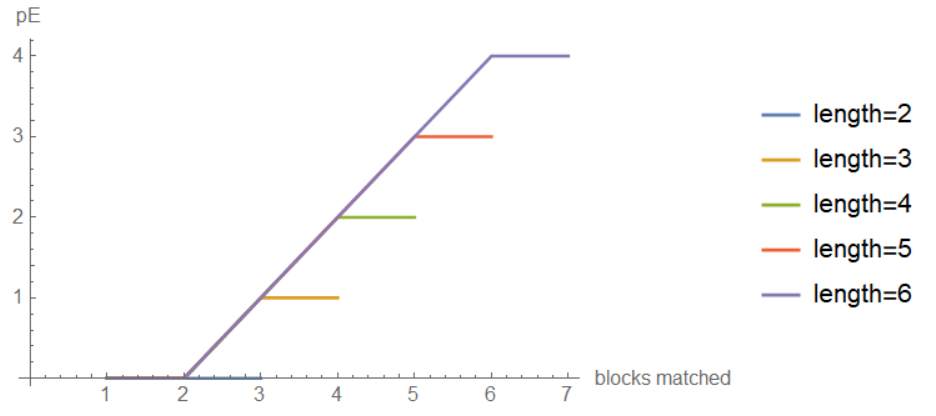
\includegraphics[width=0.8\textwidth]{images/pE.png}
}
\caption[Permitted error variable at various depths in the search tree for per filter length.]{Variable \bfit{pE} `permitted error' at various depths in the search tree (measured per block) for different filter lengths.}
\label{fig:pE_fork}
\end{figure}

Instead of forking the search path, the \gls{candidate condition} can be strengthened to suppress candidate generation for search branches with $\bfit{pE} < S-1$; This achieves the same result of forking the branches, but requires a constant-time check instead of actually forking branches.


\section{Algorithm Extensions}
\label{extensions}

The work in the \vali{} and Kucherov papers focuses primarily on the most fundamental aspects of solving the \aspop{}. Extensions exist that facilitate discovery of additional \glspl{solution}, namely \glspl{inclusion}, those brought about by consideration of \glspl{reversal}, as well as support for \gls{edit distance} as an \gls{error distance} measure. As none of these extensions change the fundamentals of the algorithms, \vali{} and Kucherov don't delve too deeply into how they should be implemented. However, the use of these extensions factors greatly into runtime, as well as requiring a significant amount of original work to implement them into the \aspop{} solver effectively.



\subsection{Edit Distance}
\label{editdistance}

\Gls{insertion} or \gls{deletion} \glspl{error} are often given the general name `\glspl{indel}'. For realistic applications in genome assembly, it is sometimes advantageous to consider \gls{edit distance}  instead of \gls{Hamming distance}), as it is defined for strings of different lengths and is more representative of the ways single-symbol errors can by physically introduced when reading genomic information. The support for these indel operations necessitates changes in both steps of the \gls{suffix filter} algorithm:

\begin{enumerate}
\item Changes to the \gls{search step}

The search procedure needs to allow branches that represent indel errors in the \gls{derivation} of match strings from the \gls{query} string. These added error operations manifest as a new set of recursive calls at each node in the search tree.

\item Changes to the \gls{verification step}

The computation to measure the error intrinsic to a \gls{candidate}’s overlap needs to be in terms of edit distance.
\end{enumerate}

Indels differentiate the lengths of the overlapping components $A$ and $B$ between the \gls{pattern} string and its \textit{match string} in the \gls{text} respectively; \Glspl{insertion} increase the length of $B$ without changing the length of $A$; \Glspl{deletion} increase the length $A$ without changing the length of $B$. These added operations necessitate that both two lengths be decoupled and stored \textit{separately} in each symbol-step of the \gls{text index}'s recursive \gls{query} search. Concepts such as \gls{string partition} size and permitted errors are defined in terms overlap length; At first glance this seems to present a circular definition, with each indel error influencing how many indel errors are permitted (by changing overlap length). Fortunately, this problem can be resolved due to the \gls{error rate} limit parameter (\bfit{e}) being strictly lower than 1, where a lengthening \gls{derived string} will always run out of errors faster than it accumulates length from errors (in the most extreme case, all errors are insertions, increasing length); This assures a hard cap for the length of derived strings.
 
In addition to complicating the algorithm conceptually and requiring further checks, the permission of indels greatly increases the branching factor of the query search, as simply more derivation branches are possible at each node in the search tree with the added operations. Thankfully, some branching \textit{rules} can be incorporated to curtail this branching factor without affecting the correctness of the algorithm. For instance, a rule could prohibit a deletion at index $N+1$ if there was an insertion at index $N$ in the same search path. Any \glspl{candidate} generated by nodes within the subtree with its root at index $N+1$ would also have been found by the subtree resulting from a \gls{substitution} at index $N$; No candidates will be overlooked by enforcing this branching rule. Many other such rules can be introduced to avoid redundant work in each search in this manner.


\subsection{Reversals}
\label{reversals}

The consideration of \glspl{reversal} comes from an application perspective. For genome assembly, \gls{read} strings in the input set $S$ are collected by reading nucleotides that are encountered when passing over a strand of \textsc{dna} or \textsc{rna} (some genomic material). In some instances, this strand is tightly bound to another companion strand, with connections at each nucleotide. Such nucleotide \textit{base pairs} always couple symmetrically and predictably, with `A' pairing with `T' and `C' pairing with `G'. Although this other strand is not read, its nucleotide sequence can be \textit{deduced} by leveraging the knowledge of its companion (which \textit{is} read). In this event, the algorithm can internally consider two strings per input string in $S$ (one given string, and one companion string) to find new overlaps involving these reversals.
 
The use of reversals has a similar impact on runtime as the use of an $S$ set twice the size. Additionally, some care must be taken as with two \textit{versions} of each read in the \gls{text}, the same solution could be found twice. Some minor bookkeeping is needed to avoid or resolve this duplication; The approach used in our implemented \aspop{} solver is detailed in Section \ref{impl:dedup}.






\subsection{Inclusions}
\label{inclusions}

\Glspl{inclusion} are a class of overlap \gls{solution} between two strings different to the suffix-prefix overlaps considered thus far. Some string $A$ is \textit{included} within some string $B$ if $A$ matches a substring of $B$. As before, this concept can be extended with the use of \glspl{error} to define a \gls{K-approximate} inclusion.
 
Knowing that two \glspl{read} came from the same genomic sequence facilitates some confidence in the correctness of the read symbols, provide redundant symbols for error correction, and helps the estimation of read `quality' (probability of misread symbols). In addition to suffix-prefix overlaps, inclusions can find such overlapping reads.
 
Extending the \aspop{} \gls{suffix filter} algorithm to also find inclusion \glspl{solution} can be done in a number of ways. One such way involves a minor change to the \gls{text index}'s search procedure. \Glspl{candidate} are now generated at the very last index of the search \gls{query} whether or not they are followed by a `\$' symbol in the \gls{text}. These special candidates would represent an occurrence of a \gls{derivation} of the \textit{entire} query string somewhere in the text (not only as the suffix to some $S$ string). The \glspl{match location} for generated candidates likely do not align with `\$' positions in the text; Thus determining to which $S$ string the match location belongs presents a minor computational challenge. Many approaches are possible, but we suggest a binary search over the known `\$' indices in the text, matching the largest `\$' index that is smaller or equal to the found index; Knowledge of which `\$' string to associate with the match location provides enough information to determine which $S$ string is associated with the found overlap, and consequently, affords the generation of a candidate;
 
Under most circumstances, allowing for inclusions greatly increases the number of candidates generated and thus increases the time taken to complete the \gls{verification step}. To see this in action, refer to Section \ref{extension_runtimes}.